\documentclass[11pt]{article}
\usepackage{geometry, times}                % See geometry.pdf to learn the layout options. There are lots.
\geometry{letterpaper}                   % ... or a4paper or a5paper or ... 
%\geometry{landscape}                % Activate for for rotated page geometry
\usepackage[parfill]{parskip}    % Activate to begin paragraphs with an empty line rather than an indent
\usepackage{fullpage, graphicx, amssymb, epstopdf, hyperref}
\hypersetup{
  colorlinks,
  linkcolor=blue,
  urlcolor=blue
}
\renewcommand{\UrlBreaks}{\do\&\do\=\do\?\do\-\do\/\do\.}
\usepackage{float}
\usepackage{verbatim}
\usepackage{pdfpages}

\DeclareGraphicsRule{.tif}{png}{.png}{`convert #1 `dirname #1`/`basename #1 .tif`.png}


%\VignetteIndexEntry{Using seawaveQ}
\usepackage[utf8]{inputenc}

\title{Vignette for seawaveQ---An R Package for Analyzing Trends in Pesticide Concentrations in Streams with a Seasonal Wave (seawave) and Adjustment for Streamflow (Q) and Other Ancillary Variables}
\author{Karen R. Ryberg and Aldo V. Vecchia}
\date{\today}                                % Activate to display a given date or no date

\usepackage{/Library/Frameworks/R.framework/Resources/share/texmf/tex/latex/Sweave}
\begin{document}
\maketitle
\tableofcontents

\section{Introduction}

This R package, \textbf{seawaveQ}, is designed  for fitting a parametric regression model for assessing variability and trends in pesticide concentration in streams and was developed by Vecchia and others (2008), and subsequently refined and referred to as the ``seawave-Q'' model in several trend analyses (Ryberg and others, 2010; Sullivan and others, 2009; Vecchia and others, 2009).  In these publications, ``seawave-Q'' stands for seasonal wave (seawave) with adjustment for streamflow (Q).  The model was developed to ``handle a number of difficulties often found in pesticide data, such as strong seasonality in response to use patterns, high numbers of concentrations below laboratory reporting levels (RLs), complex relations between streamflow and concentration, and intermittent or changing sampling frequencies (both inter-annually and intra-annually)'' (Vecchia and others, 2008).  This R package provides a standardized methodology for fitting the seawave-Q model and makes the trend analysis method widely available for use by others. In addition, several enhancements to the seawave-Q model have been included such as: procedures for preparing and summarizing input data; flexibility to include other explanatory variables besides streamflow; graphical methods for assessing model fit; and additional model outputs.    A flow chart showing how the various function in the package work together is shown in figure 1 of the U.S. Geological Survey Open-File Report documenting this package (Ryberg and Vecchia, 2013). 

The statistical methodology for the seawave-Q model is described in Vecchia and others (2008) and in the U.S. Geological Survey Open-File Report documenting this package (Ryberg and Vecchia, 2013).   Users new to this model should read both of those documents before applying the model to their own data.  An important part of the model and the output shown below is the seasonal wave. The seasonal wave is a periodic (with a period of 1 year) solution to a differential equation (Vecchia and others, 2008) that has a pulse input function, a seasonal shift that determines the time at which the seasonal wave reaches its maximum, and a model half-life.

\section{Input Data}

The seawaveQ model needs two types of input data.  The first is the the water-quality sample data including dates, the concentration data, and qualification codes, indicating which values are censored (less than a long-term method detection level).  The second type of data is the continuous ancillary data used in the model, such as streamflow anomalies (Ryberg and Vecchia, 2012).  These ancillary data are also used to produce a continuous estimate of pesticide concentration.  Examples of the necessary format of these two data sets are provided and documented in the package.  The following code shows how to access the example data.
\vspace{5 mm}

\begin{Schunk}
\begin{Sinput}
> # load waterData package, assuming it has already been installed on the system
> library(seawaveQ)
> # load example data that comes with the package
> data(swData)
> # show first few rows of water-quality data for Missouri River at Omaha, Nebraska
> head(qwMoRivOmaha)
\end{Sinput}
\begin{Soutput}
     staid      dates times R04035 P04035 R04037 P04037 R04041 P04041 R39415 P39415
1 06610000 1996-01-13  1130      <  0.004      _  0.024      <  0.008      _  0.006
2 06610000 1996-02-13  1200      <  0.004      E  0.005      <  0.008      _  0.200
3 06610000 1996-03-13  1000      E  0.005      E  0.004      <  0.008      _  0.026
4 06610000 1996-03-28  1030      <  0.004      E  0.005      _  0.009      _  0.026
5 06610000 1996-04-09  1100      _  0.007      E  0.006      _  0.014      _  0.075
6 06610000 1996-04-23  1000      <  0.004      <  0.004      _  0.012      _  0.040
  R46342 P46342 R82630 P82630 R82661 P82661 R82668 P82668
1      <  0.003      _  0.029      <  0.003      _  0.008
2      <  0.003      <  0.007      <  0.003      _  0.007
3      <  0.003      <  0.007      <  0.003      E  0.004
4      <  0.003      <  0.007      <  0.003      _  0.008
5      E  0.003      <  0.007      <  0.003      _  0.009
6      <  0.003      <  0.007      <  0.003      <  0.002
\end{Soutput}
\begin{Sinput}
> # get a description of the data including definitions of the columns
> # by viewing the help documentation
> ?qwMoRivOmaha
\end{Sinput}
\end{Schunk}

Optionally, functions have been provided to plot concentration data.  These functions produce scatter plots and box plots that indicate or take into account the censored, less than, values.  The functions are \textit{cenScatPlot} and \textit{rosBoxPlot} and examples of their use follow.  The box plots are generated using the function \textit{ros}, regression on order statistics, in the R package \textbf{NADA} (Lee, 2012).  It is an implementation of a regression on order statistics designed for multiply-censored analytical-chemistry data  (Helsel, 2005). 
\vspace{5 mm}

\begin{figure}[H]
\centering
%\setkeys{Gin}{width=1.45\textwidth}
\begin{Schunk}
\begin{Sinput}
> # scatter plot showing unqualified, estimated, and censored  values
> cenScatPlot(qwMoRivOmaha, pname="04035")
\end{Sinput}
\end{Schunk}
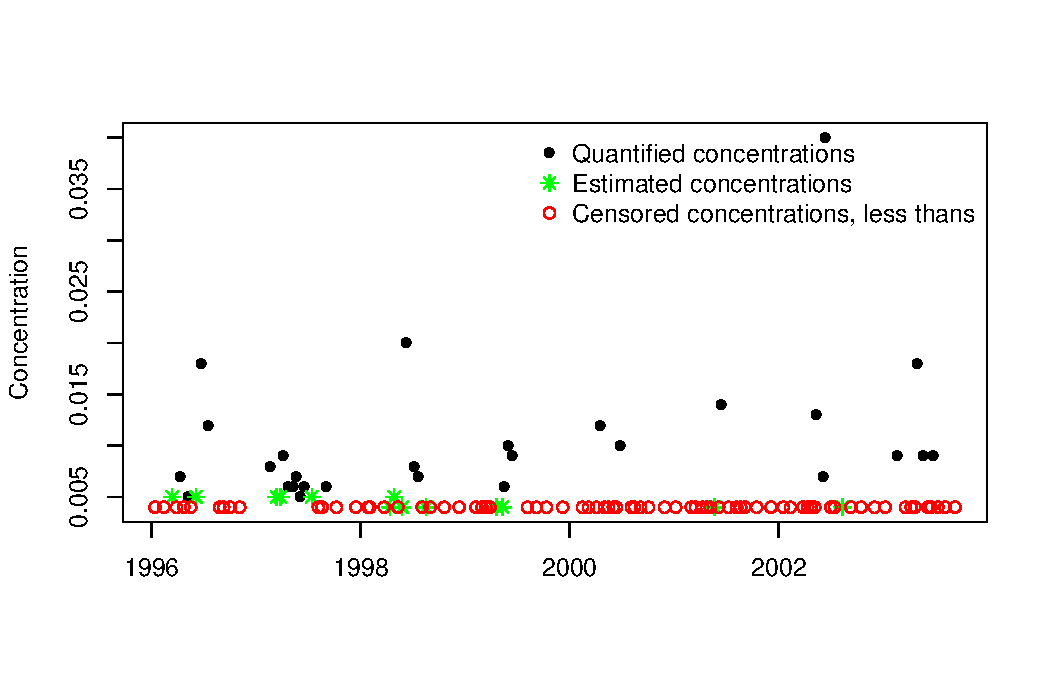
\includegraphics{vignette-002}
\end{figure}

\begin{figure}[H]
\centering
%\setkeys{Gin}{width=1.45\textwidth}
\begin{Schunk}
\begin{Sinput}
> # scatter plot with many additional plotting arguments
> # these options provide a plot closer to the plotting standards
> #  of the U.S. Geological Survey however, these plots may not 
> # meet all U.S. Geological Survey publication requirements
> par(las=1, tcl=0.5)
> cenScatPlot(qwMoRivOmaha, pname="04035", 
+                        site="06610000 Missouri River at Omaha, Neb.",
+                        ylabel="Simazine concentration, in micrograms per liter",
+                        legcex=0.7, qwcols=c("R", "P"), ylim=c(0,0.1), yaxs="i", 
+                        cex.lab=0.9, cex.axis=0.9, xlim=c(as.Date("1996-01-01"), 
+                        as.Date("2004-01-01")), xaxs="i", xaxt="n")
> axdates <- c("1996-01-01", "1998-01-01", "2000-01-01", 
+                        "2002-01-01", "2004-01-01")
> axis(1, as.Date(axdates), 
+                        labels=c("1996", "1998", "2000", "2002", "2004"), cex.axis=0.9)
\end{Sinput}
\end{Schunk}
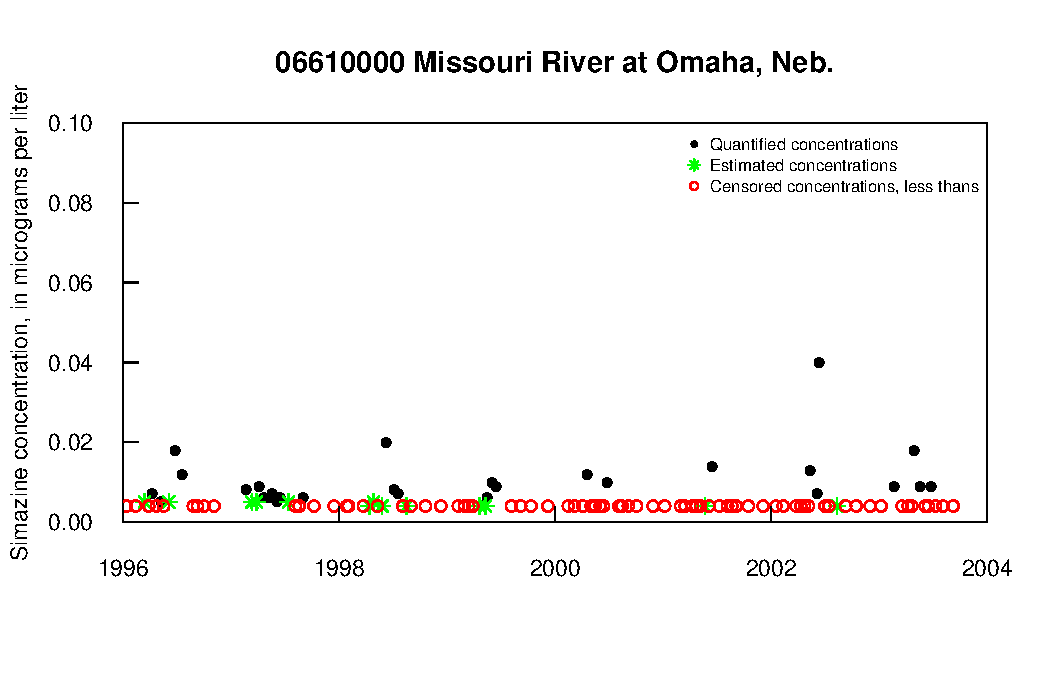
\includegraphics{vignette-003}
\end{figure}

\begin{figure}[H]
\centering
%\setkeys{Gin}{width=1.45\textwidth}
\begin{Schunk}
\begin{Sinput}
> # simple box plots of water-quality concentrations
> rosBoxPlot(qwMoRivOmaha, qwcols=c("R", "P"))
\end{Sinput}
\end{Schunk}
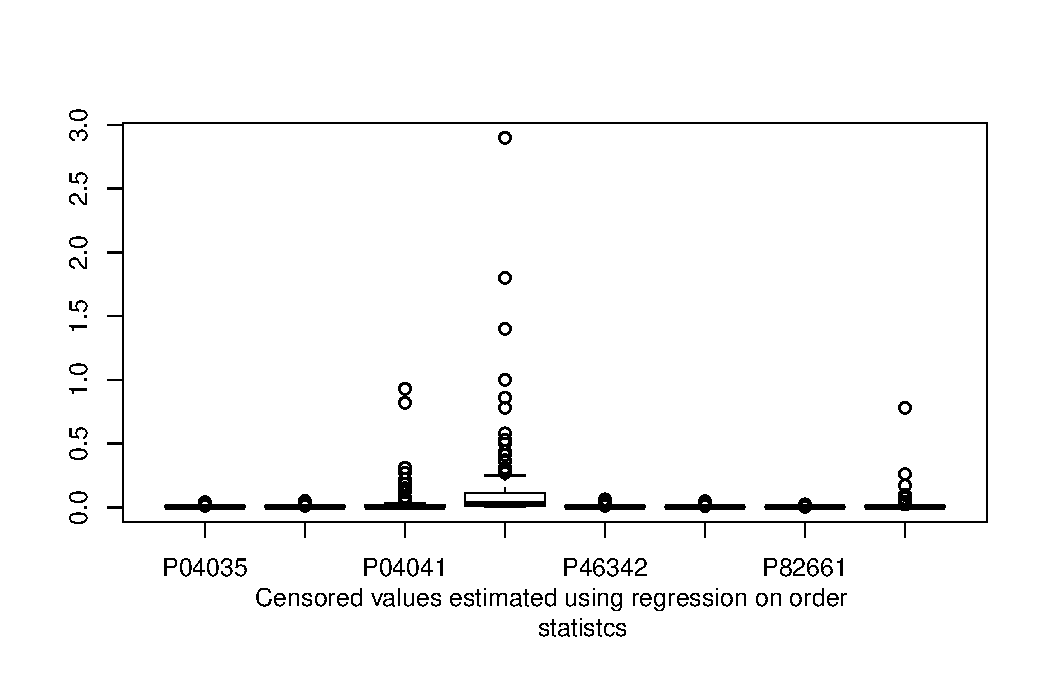
\includegraphics{vignette-004}
\end{figure}

\begin{figure}[H]
\centering
%\setkeys{Gin}{width=1.45\textwidth}
\begin{Schunk}
\begin{Sinput}
> # same boxplot function with many additional plotting arguments
> rosBoxPlot(qwMoRivOmaha, site="06610000 Missouri River at Omaha, Neb.",
+                      log="y", yaxt="n", ylim=c(0.000001, 10), qwcols=c("R", "P"), 
+                      ylab=c("Concentration, micrograms per liter"), col="skyblue1",
+                      cex.axis=0.7, cex.sub=0.8, 
+                      par(tcl=0.5, las=1, yaxs="i", mgp=c(3,0.5,0), mar=c(5,5,2,2), 
+                      cex.main=0.9))
> axis(2, at=c(0.000001, 0.00001, 0.0001, 0.001, 0.01, 0.1, 1, 10),
+ labels=c("0.000001", "0.00001", "0.0001", "0.001", "0.01",
+ "0.1", "1", "10"), cex.axis=0.7)
\end{Sinput}
\end{Schunk}
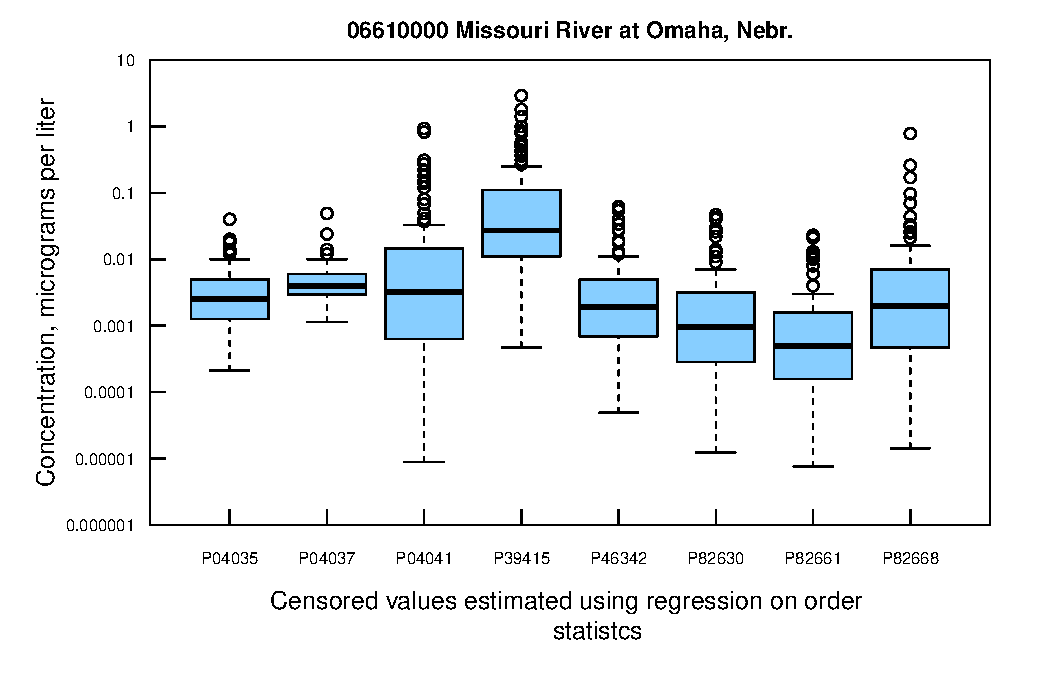
\includegraphics{vignette-005}
\end{figure}

The second data set needed is the one containing the continuous ancillary data for building the model that describes pesticide concentrations.  
\vspace{5 mm}

\begin{Schunk}
\begin{Sinput}
> data(swData)
> # show last few rows of water-quality data for Missouri River at Omaha, Nebraska
> tail(cqwMoRivOmaha)
\end{Sinput}
\begin{Soutput}
        staid      dates dflow     flowa30      flowa1 dsed     seda30       seda1
2917 06610000 2003-09-25 29200 -0.09433312 -0.00527612  176 -0.1546322 -0.10766231
2918 06610000 2003-09-26 28800 -0.09268448 -0.01291513  177 -0.1566163 -0.10321762
2919 06610000 2003-09-27 28700 -0.09102975 -0.01608045  181 -0.1579888 -0.09213983
2920 06610000 2003-09-28 28700 -0.08926147 -0.01784872  184 -0.1588294 -0.08416002
2921 06610000 2003-09-29 28600 -0.08754373 -0.02108233  189 -0.1586754 -0.07267005
2922 06610000 2003-09-30 28700 -0.08577546 -0.02133474  201 -0.1569162 -0.04769499
\end{Soutput}
\begin{Sinput}
> # get a description of the data including definitions of the columns
> # by viewing the help documentation
> ?cqwMoRivOmaha
\end{Sinput}
\end{Schunk}
\vspace{5 mm}

In this case, the continuous ancillary data includes daily streamflow (dflow) and daily sediment concentration (dsed), as well as the 30-day and 1-day streamflow (flowa30 and flowa1) and sediment (seda30 and seda1) anomalies.  (The anomalies were calculated using the \textbf{waterData} package for R.)

In order to build a model using one or more of these ancillary variables as explanatory variables for pesticide concentration, the continuous ancillary variables need to be associated with the water-quality samples.  The function \textit{combineData} will combine water-quality sample data and continuous (daily) ancillary variables and drop unnecessary columns.  One needs to specify the water-quality sample data, the continuous ancillary data, and the columns representing the station identifier, the data, the qualification code columns, and the concentration columns as shown in the following code.
\vspace{5 mm}

\begin{Schunk}
\begin{Sinput}
> data(swData)
> MoRivOmaha<-combineData(qwdat=qwMoRivOmaha, cqwdat=cqwMoRivOmaha,
+ qwcols=c("staid", "dates", "R", "P"))
> # view combined data set
> head(MoRivOmaha)
\end{Sinput}
\begin{Soutput}
     staid      dates R04035 P04035 R04037 P04037 R04041 P04041 R39415 P39415
1 06610000 1996-01-13      <  0.004      _  0.024      <  0.008      _  0.006
2 06610000 1996-02-13      <  0.004      E  0.005      <  0.008      _  0.200
3 06610000 1996-03-13      E  0.005      E  0.004      <  0.008      _  0.026
4 06610000 1996-03-28      <  0.004      E  0.005      _  0.009      _  0.026
5 06610000 1996-04-09      _  0.007      E  0.006      _  0.014      _  0.075
6 06610000 1996-04-23      <  0.004      <  0.004      _  0.012      _  0.040
  R46342 P46342 R82630 P82630 R82661 P82661 R82668 P82668 dflow      flowa30
1      <  0.003      _  0.029      <  0.003      _  0.008 25800 -0.111771936
2      <  0.003      <  0.007      <  0.003      _  0.007 30500 -0.155914620
3      <  0.003      <  0.007      <  0.003      E  0.004 32600 -0.043752697
4      <  0.003      <  0.007      <  0.003      _  0.008 42400 -0.004315925
5      E  0.003      <  0.007      <  0.003      _  0.009 50300  0.073100169
6      <  0.003      <  0.007      <  0.003      <  0.002 48800  0.126711034
        flowa1 dsed      seda30       seda1
1 -0.041600453  255  0.04313266 -0.14439969
2  0.075222364  312  0.02706313 -0.04071575
3 -0.008021798  236 -0.02856792 -0.10632729
4  0.066689687  609  0.01503934  0.26177074
5  0.063475721  528  0.13734452  0.07748219
6 -0.003283307  368  0.23175763 -0.17371703
\end{Soutput}
\end{Schunk}

\section{Fitting the seawaveQ Model}

One can now fit the seawaveQ model using the data explored and combined in the previous code examples.  The follow code fits three different seawaveQ models (with differing continuous ancillary variables) for two pesticides in the data set.  The pesticides are 04035, simazine, and 04041, cyanazine.  See the help documentation for further information about the function arguments shown and additional arguments.
\vspace{5 mm}

\begin{Schunk}
\begin{Sinput}
> myfit1 <- fitswavecav(cdat=modMoRivOmaha, cavdat=cqwMoRivOmaha,
+ tanm="myfit1", pnames=c("04035", "04041"), yrstart=1995,
+ yrend=2003, tndbeg=1995, tndend=2003, iwcav=c("flowa30", "flowa1"),
+ dcol="dates", qwcols=c("R","P"))
> myfit2 <- fitswavecav(cdat=modMoRivOmaha, cavdat=cqwMoRivOmaha,
+ tanm="myfit2", pnames=c("04035", "04041"), yrstart=1995,
+ yrend=2003, tndbeg=1995, tndend=2003, iwcav=c("seda30", "seda1"),
+ dcol="dates", qwcols=c("R","P"))
> myfit3 <- fitswavecav(cdat=modMoRivOmaha, cavdat=cqwMoRivOmaha,
+ tanm="myfit3", pnames=c("04035", "04041"), yrstart=1995,
+ yrend=2003, tndbeg=1995, tndend=2003, iwcav=c("flowa30", "flowa1",
+ "seda30", "seda1"), dcol="dates", qwcols=c("R","P"))
\end{Sinput}
\end{Schunk}

\section{Model Output}
The model fitting process finds the best pulse input function and model half-life for the concentration data and uses survival regression to fit a regression model.  Three types of output are provided: 1) a list, the first element being a data frame with information about the model and its parameters, the second element being the survival regression summary; 2) text files showing a summary of the survival regression results, like the second element of the list, but with  additional measures of model quality and information about the R session; and 3) a pdf file of plots showing the model, trend, and diagnostic plots.  The data frame results for the three models for simazine and cyanazine are shown below.
\vspace{5 mm}

\begin{Schunk}
\begin{Sinput}
> # get the first element of the list for each model/constituent combination
> # the data frame with information about each model/constituent combination
> myfit1[[1]]
\end{Sinput}
\begin{Soutput}
  pname mclass jmod hlife   cmaxt     scl    loglik     cint   cwave     ctnd
1 04035      1    3     1 0.48087 0.27216 -32.82218 -2.49433 0.55360 -0.02850
2 04041      1    4     3 0.48087 0.42843 -43.90813 -2.27666 2.16327 -0.25063
  cflowa30 cflowa1   seint  sewave   setnd seflowa30 seflowa1
1  0.05509 2.09772 0.04908 0.11183 0.02191   0.30734  0.46967
2  0.00587 2.95546 0.08622 0.26127 0.03775   0.52071  0.78638
\end{Soutput}
\begin{Sinput}
> myfit2[[1]]
\end{Sinput}
\begin{Soutput}
  pname mclass jmod hlife   cmaxt     scl    loglik     cint   cwave     ctnd
1 04035      1    5     3 0.48087 0.24680 -24.33186 -2.68415 0.79622 -0.02478
2 04041      1    3     2 0.48087 0.41225 -40.46237 -2.13390 1.57758 -0.22234
  cseda30  cseda1   seint  sewave   setnd seseda30 seseda1
1 0.25178 0.59654 0.06853 0.18670 0.01637  0.17377 0.10251
2 1.14307 0.62894 0.07579 0.19086 0.02996  0.29031 0.18224
\end{Soutput}
\begin{Sinput}
> myfit3[[1]]
\end{Sinput}
\begin{Soutput}
  pname mclass jmod hlife   cmaxt     scl    loglik     cint   cwave     ctnd
1 04035      1    5     3 0.48087 0.24625 -23.83840 -2.67858 0.76537 -0.01883
2 04041      1    3     2 0.48087 0.39523 -38.65962 -2.08402 1.70493 -0.24244
  cflowa30  cflowa1 cseda30  cseda1   seint  sewave   setnd seflowa30 seflowa1
1  0.17756 -0.36824 0.22666 0.66734 0.06725 0.18450 0.01991   0.30663  0.64400
2 -0.57741  1.53888 1.04420 0.29466 0.07942 0.20191 0.03459   0.50123  1.12286
  seseda30 seseda1
1  0.20480 0.15247
2  0.31298 0.27108
\end{Soutput}
\begin{Sinput}
> # get the second element of the list for each model/constituent combination
> # the survival regression summary for each model/constituent combination
> myfit1[[2]]
\end{Sinput}
\begin{Soutput}
[[1]]

Call:
survreg(formula = Surv(time = clogtmp, time2 = indcen, type = "left") ~ 
    xxxmat - 1, dist = "gaussian")
                Value Std. Error       z        p
xxxmatintcpt  -2.4943     0.0491 -50.826 0.00e+00
xxxmatwavest   0.5536     0.1118   4.950 7.41e-07
xxxmattndlin  -0.0285     0.0219  -1.301 1.93e-01
xxxmatflowa30  0.0551     0.3073   0.179 8.58e-01
xxxmatflowa1   2.0977     0.4697   4.466 7.96e-06
Log(scale)    -1.3013     0.1205 -10.797 3.57e-27

Scale= 0.272 

Gaussian distribution
Loglik(model)= -32.8   Loglik(intercept only)= -60.9
	Chisq= 56.1 on 4 degrees of freedom, p= 1.9e-11 
Number of Newton-Raphson Iterations: 5 
n= 115 


[[2]]

Call:
survreg(formula = Surv(time = clogtmp, time2 = indcen, type = "left") ~ 
    xxxmat - 1, dist = "gaussian")
                 Value Std. Error        z         p
xxxmatintcpt  -2.27666     0.0862 -26.4055 1.19e-153
xxxmatwavest   2.16327     0.2613   8.2799  1.23e-16
xxxmattndlin  -0.25063     0.0377  -6.6393  3.15e-11
xxxmatflowa30  0.00587     0.5207   0.0113  9.91e-01
xxxmatflowa1   2.95546     0.7864   3.7583  1.71e-04
Log(scale)    -0.84763     0.1038  -8.1685  3.12e-16

Scale= 0.428 

Gaussian distribution
Loglik(model)= -43.9   Loglik(intercept only)= -103.7
	Chisq= 119.63 on 4 degrees of freedom, p= 0 
Number of Newton-Raphson Iterations: 6 
n= 115 
\end{Soutput}
\begin{Sinput}
> myfit2[[2]]
\end{Sinput}
\begin{Soutput}
[[1]]

Call:
survreg(formula = Surv(time = clogtmp, time2 = indcen, type = "left") ~ 
    xxxmat - 1, dist = "gaussian")
               Value Std. Error      z        p
xxxmatintcpt -2.6841     0.0685 -39.17 0.00e+00
xxxmatwavest  0.7962     0.1867   4.26 2.00e-05
xxxmattndlin -0.0248     0.0164  -1.51 1.30e-01
xxxmatseda30  0.2518     0.1738   1.45 1.47e-01
xxxmatseda1   0.5965     0.1025   5.82 5.90e-09
Log(scale)   -1.3992     0.1184 -11.82 3.16e-32

Scale= 0.247 

Gaussian distribution
Loglik(model)= -24.3   Loglik(intercept only)= -60.9
	Chisq= 73.08 on 4 degrees of freedom, p= 5.1e-15 
Number of Newton-Raphson Iterations: 6 
n= 115 


[[2]]

Call:
survreg(formula = Surv(time = clogtmp, time2 = indcen, type = "left") ~ 
    xxxmat - 1, dist = "gaussian")
              Value Std. Error      z         p
xxxmatintcpt -2.134     0.0758 -28.15 2.10e-174
xxxmatwavest  1.578     0.1909   8.27  1.39e-16
xxxmattndlin -0.222     0.0300  -7.42  1.15e-13
xxxmatseda30  1.143     0.2903   3.94  8.24e-05
xxxmatseda1   0.629     0.1822   3.45  5.58e-04
Log(scale)   -0.886     0.1029  -8.61  7.00e-18

Scale= 0.412 

Gaussian distribution
Loglik(model)= -40.5   Loglik(intercept only)= -103.7
	Chisq= 126.52 on 4 degrees of freedom, p= 0 
Number of Newton-Raphson Iterations: 6 
n= 115 
\end{Soutput}
\begin{Sinput}
> myfit3[[2]]
\end{Sinput}
\begin{Soutput}
[[1]]

Call:
survreg(formula = Surv(time = clogtmp, time2 = indcen, type = "left") ~ 
    xxxmat - 1, dist = "gaussian")
                Value Std. Error       z        p
xxxmatintcpt  -2.6786     0.0673 -39.828 0.00e+00
xxxmatwavest   0.7654     0.1845   4.148 3.35e-05
xxxmattndlin  -0.0188     0.0199  -0.946 3.44e-01
xxxmatflowa30  0.1776     0.3066   0.579 5.63e-01
xxxmatflowa1  -0.3682     0.6440  -0.572 5.67e-01
xxxmatseda30   0.2267     0.2048   1.107 2.68e-01
xxxmatseda1    0.6673     0.1525   4.377 1.20e-05
Log(scale)    -1.4014     0.1188 -11.800 3.92e-32

Scale= 0.246 

Gaussian distribution
Loglik(model)= -23.8   Loglik(intercept only)= -60.9
	Chisq= 74.06 on 6 degrees of freedom, p= 6e-14 
Number of Newton-Raphson Iterations: 6 
n= 115 


[[2]]

Call:
survreg(formula = Surv(time = clogtmp, time2 = indcen, type = "left") ~ 
    xxxmat - 1, dist = "gaussian")
               Value Std. Error      z         p
xxxmatintcpt  -2.084     0.0794 -26.24 9.36e-152
xxxmatwavest   1.705     0.2019   8.44  3.07e-17
xxxmattndlin  -0.242     0.0346  -7.01  2.39e-12
xxxmatflowa30 -0.577     0.5012  -1.15  2.49e-01
xxxmatflowa1   1.539     1.1229   1.37  1.71e-01
xxxmatseda30   1.044     0.3130   3.34  8.49e-04
xxxmatseda1    0.295     0.2711   1.09  2.77e-01
Log(scale)    -0.928     0.1035  -8.97  3.00e-19

Scale= 0.395 

Gaussian distribution
Loglik(model)= -38.7   Loglik(intercept only)= -103.7
	Chisq= 130.12 on 6 degrees of freedom, p= 0 
Number of Newton-Raphson Iterations: 6 
n= 115 
\end{Soutput}
\begin{Sinput}
> 
\end{Sinput}
\end{Schunk}
\vspace{5 mm}
The first item of the list, the data frame, contains information about each model including the pesticide analyzed; the model class (an option in seawaveQ that is not currently implemented but that will provide additional model options in the future); the choice of model or pulse input function, an integer 1 through 14; the model half-life in months, an integer, 1 to 4 months; the decimal season of highest concentration; the scale factor from the survreg.object; the log-likelihood for the model; the coefficient for the model intercept; the coefficient for the seasonal wave; the coefficient for the trend component of the model; 0 or more values representing coefficients for the continuous ancillary variables; the standard error for the intercept; the standard error for the seasonal wave; the standard error for the trend; and 0 or more columns representing standard errors for the continuous ancillary variables.

The second item of the list is provided so that users could extract the attributes of the survival regression summary programmatically (rather than viewing them in the text file) and create  their own summaries or plots of the results.

\begin{Schunk}
\begin{Sinput}
> attributes(myfit1[[2]][[1]])
\end{Sinput}
\begin{Soutput}
$names
 [1] "call"         "df"           "loglik"       "iter"         "idf"         
 [6] "scale"        "coefficients" "var"          "table"        "correlation" 
[11] "parms"        "n"            "chi"          "robust"      

$class
[1] "summary.survreg"
\end{Soutput}
\begin{Sinput}
> myfit1[[2]][[1]]$n
\end{Sinput}
\begin{Soutput}
[1] 115
\end{Soutput}
\begin{Sinput}
> myfit1[[2]][[1]]$table
\end{Sinput}
\begin{Soutput}
                    Value Std. Error           z            p
xxxmatintcpt  -2.49432580 0.04907615 -50.8256204 0.000000e+00
xxxmatwavest   0.55360325 0.11183213   4.9503061 7.409685e-07
xxxmattndlin  -0.02849686 0.02190660  -1.3008343 1.933152e-01
xxxmatflowa30  0.05509435 0.30734075   0.1792615 8.577324e-01
xxxmatflowa1   2.09771895 0.46966962   4.4663714 7.955747e-06
Log(scale)    -1.30134822 0.12053152 -10.7967458 3.566195e-27
\end{Soutput}
\begin{Sinput}
> 
\end{Sinput}
\end{Schunk}
\vspace{5 mm}

The text file for the first of the function calls above is inserted here as an example.  Users may run the model fitting code themselves and view the resulting text files for all three models.  The results for all three are too long to include in this vignette.

\vspace{5 mm}

\verbatiminput{myfit1_survregCall.txt}%

\vspace{5 mm}

The plots written to a pdf file for the first pesticide, 04035, simazine, in the first model, myfit1, are included below.  As with the text results, the plots for all three models and all pesticides are too numerous to include here.  Users are encouraged to run the code themselves and examine all of the plots.

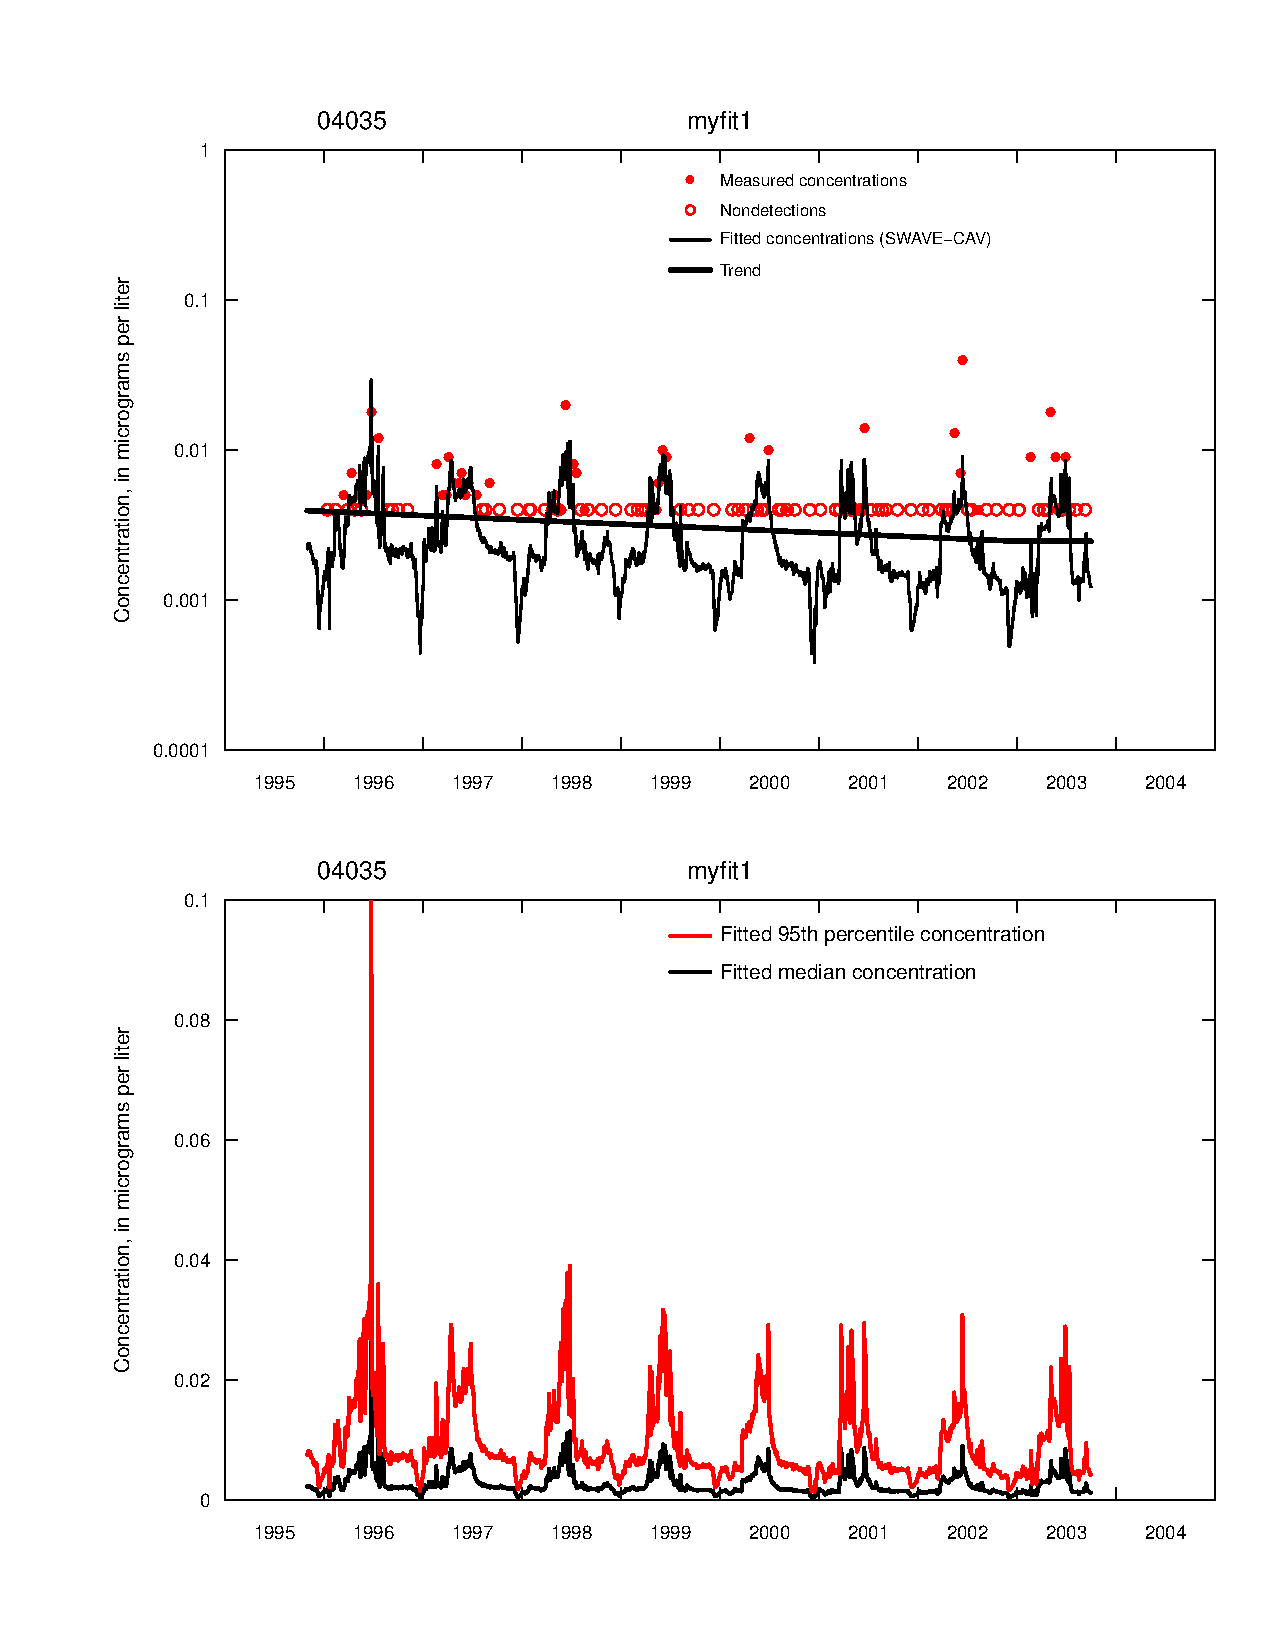
\includepdf[pages={-}]{myfit104035.pdf}

\vspace{5 mm}

The plotting position used for representing censored values in the model plots (produced by the internal function \textit{seawaveQPlots} further described in the package help documentation) is an important consideration for interpreting model fit.  Plotting values obtained by using the censoring limit, or something smaller such as one-half of the censoring limit, produce plots that are difficult to interpret if there are a large number of censored values.  Therefore, to make the plots more representative of diagnostic plots used for standard (non-censored) regression,  a method for substituting randomized residuals in place of censored residuals was used.   If a log-transformed concentration is censored at a particular limit, $logC < L$, then the residual for that concentration is censored as well, $logC - fitted(logC) < L - fitted(logC) = rescen)$.  In that case, a randomized residual was generated from a conditional normal distribution:
\begin{verbatim}
	resran  <-  scl * qnorm(runif(1) * pnorm(rescen / scl))
\end{verbatim}
where \textit{scl} is the scale parameter from the survival regression model, \textit{pnorm} is the R function for computing cumulative normal probabilities, \textit{runif} is the R function for generating a random variable from the uniform distribution, and \textit{qnorm} is the R function for computing quantiles of the normal distribution.  Under the assumption that the model residuals are uncorrelated, normally distributed random variables with mean zero and standard deviation scl, the randomized residuals generated in this manner are an unbiased sample of the true (but unknown) residuals for the censored data.  The plotting position used a censored concentration is $fitted(logC) + resran$.  Note that each time a new model fit is performed, a new set of randomized residuals is generated and thus the plotting positions for censored values can change.

\section{References}
Helsel, D.R., 2005, Nondetects and data analysis: New York, John Wiley and Sons.

Lee, Lopaka, 2012, Nondetects and data analysis for environmental data: R package version 1.5-4,
\url{http://CRAN.R-project.org/package=NADA}.

Ryberg, K.R. and Vecchia, A.V., 2006, Water-quality trend analysis and sampling design for the Devils Lake Basin, North Dakota, January 1965 through September 2003: U.S. Geological Survey Scientific Investigations Report 2006--5238, 64 p.,  accessed May 1, 2012, at \url{http://pubs.usgs.gov/sir/2006/5238/}.

Ryberg, K.R. and Vecchia, A.V., 2012, waterData---An R package for retrieval, analysis, and anomaly calculation of daily hydrologic time series data, version 1.0: U.S. Geological Survey Open-File Report 2012--1168, 8 p., accessed March 1, 2013, at \url{http://pubs.usgs.gov/of/2012/1168/}.

Ryberg, K.R., and Vecchia, A.V., 2013, seawaveQ---An R Package for Analyzing Trends in Pesticide Concentrations in Streams with a Seasonal Wave (seawave) and Adjustment for Streamflow (Q) and Other Ancillary Variables: U.S. Geological Survey Open-File Report 2013-XXXX, XX p.

Ryberg, K.R., Vecchia, A.V., Martin, J.D., and Gilliom, R.J., 2010, Trends in pesticide concentrations in urban streams in the United States, 1992-2008: U.S. Geological Survey Scientific Investigations Report 2010--5139, 101 p.,  accessed May 1, 2012, at \url{http://pubs.usgs.gov/sir/2010/5139/}.

Sullivan, D.J., Vecchia, A.V., Lorenz, D.L., Gilliom, R.J., and Martin, J.D., 2009, Trends in pesticide concentrations in corn-belt streams, 1996--2006: U.S. Geological Survey Scientific Investigations Report 2009--5132, 75 p.,  accessed May 1, 2012, at \url{http://pubs.usgs.gov/sir/2009/5132/}.

Vecchia, A.V., 2005, Water-quality trend analysis and sampling design for streams in the Red River of the North Basin, Minnesota, North Dakota, and South Dakota, 1970--2001: U.S. Survey Scientific Investigations Report 2005--5224, 54 p., accessed May 1, 2012, at \url{http://pubs.usgs.gov/sir/2005/5224/}.

Vecchia, A.V., Gilliom, R.J., Sullivan, D.J., Lorenz, D.L., and Martin, J.D., 2009, Trends in concentrations and use of agricultural herbicides for Corn Belt rivers, 1996--2006:  Environmental Science and Technology, v. 43, p. 9,096-9,102, accessed May 1, 2012, at \url{http://water.usgs.gov/nawqa/pubs/es902122j.pdf}.

Vecchia, A.V., Martin, J.D., and Gilliom, R.J., 2008, Modeling variability and trends in pesticide concentrations in streams: Journal of the American Water Resources Association, v. 44, no. 5, pp. 1,308-1,324, accessed May 1, 2012, at \url{http://dx.doi.org/10.1111/j.1752-1688.2008.00225.x}.

\end{document}  
